\newpage
\section{Information flow}
\label{sec:information_flow}

The client will always be the initiator in either requesting data from the
server or sending data. 

\begin{figure}[h!]
    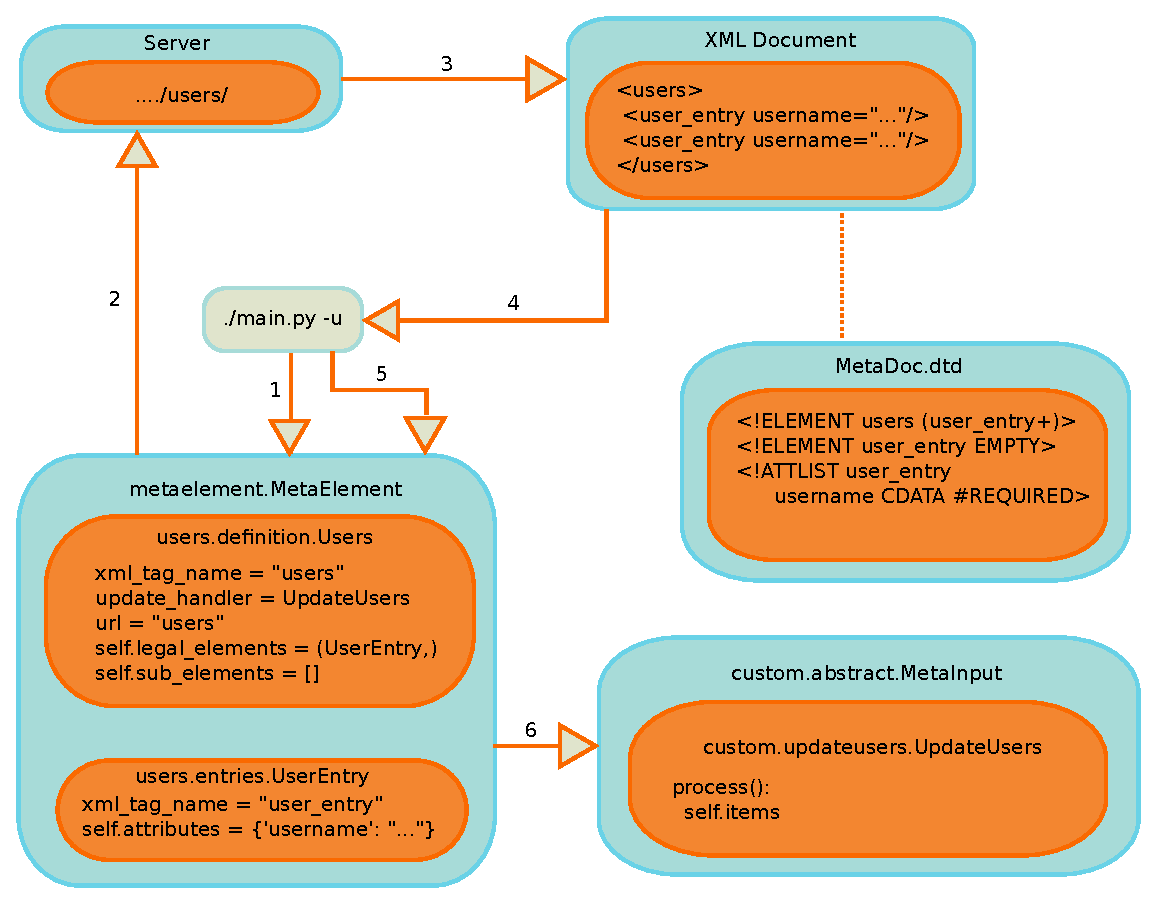
\includegraphics[width=\textwidth]{img/xml_flow}
    \caption{Information flow when requesting user list with MetaDoc}
    \label{fig:information_flow}
\end{figure}

Figure \ref{fig:information_flow} shows how information passes when a client
requests a user list. The steps are as follows:

\begin{enumerate}
    \item
        \texttt{main.py} is run with the handle \textbf{-u}, which will check
        \texttt{users.definition.Users} for which URL to access on the server
        to retrieve the information.
    \item
        A request is sent to the server to retrieve the information.
    \item
        The server creates an \gls{xml} document with a list of users for the
        site.
        
        The \gls{xml} document sent is defined by the MetaDoc \gls{dtd}.
    \item
        \texttt{main.py} recieves the \gls{xml} document, checks that it is
        valid according to the \gls{dtd}. 
    \item
        If the \gls{xml} document passes validation, an instance of
        \texttt{users.definition.Users} is created, and an instance of
        \texttt{users.entries.UserEntry} is created for each
        \texttt{<user\_entry>} in the \gls{xml} document.

        \texttt{users.definition.Users} and \texttt{users.entries.UserEntry}
        may validate attributes and refuse to create any elements where
        attribute validation does not pass.
    \item
        The list of validated \texttt{users.entries.UserEntry} instances is
        placed within \texttt{self.items} for an
        \texttt{custom.updateusers.UpdateUsers} instance, and the
        \texttt{process()} function is called for the processing of the user
        list.
\end{enumerate}

\subsection{Validation}

\begin{figure}[h!]
    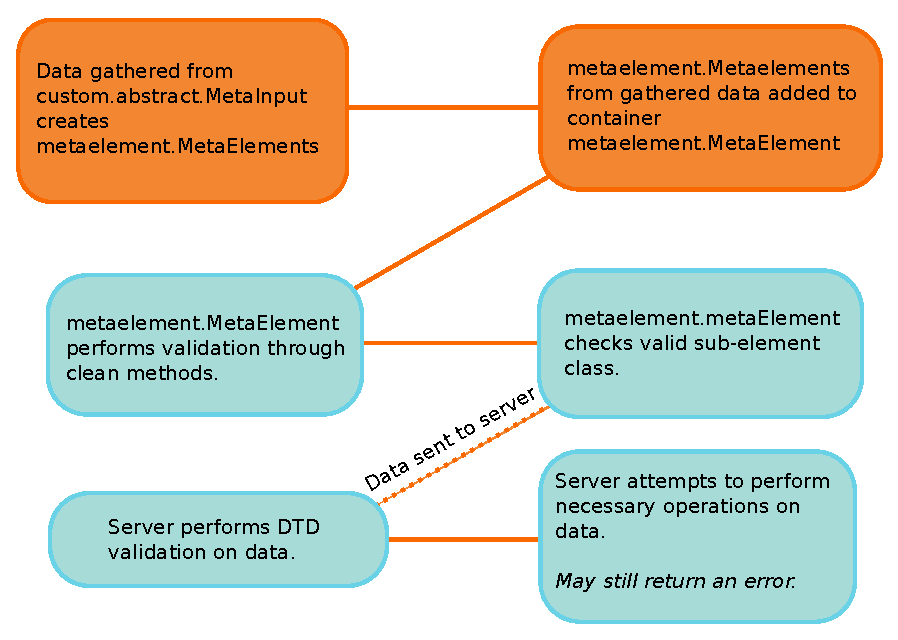
\includegraphics[width=\textwidth]{img/site_information_flow}
    \caption{Shows validation procedures when data is passed from client to
    server}
    \label{fig:site_information_flow}
\end{figure}

\begin{figure}[h!]
    \includegraphics[width=\textwidth]{img/server_information_flow}
    \caption{Shows validation procedures when data is passed from server to
    client}
    \label{fig:server_information_flow}
\end{figure}
